\documentclass[11pt,a4paper]{article}
\usepackage[margin=1in]{geometry}
\usepackage[T1]{fontenc}
\usepackage[utf8]{inputenc}
\usepackage{lmodern}
\usepackage{hyperref}
\usepackage{enumitem}
\usepackage{xurl}
\usepackage{tikz}
\usepackage{float}
\usetikzlibrary{arrows.meta, positioning, shapes.geometric}
\hypersetup{colorlinks=true,linkcolor=blue,urlcolor=blue}
\newcommand{\codepath}[1]{\path{#1}}
\tikzset{
  box/.style={rectangle,draw,rounded corners,align=center,inner sep=3pt,minimum width=44mm},
  decision/.style={diamond,draw,aspect=2.2,align=center,inner sep=2pt},
  line/.style={-Latex}
}

\title{Phase-2 Spike: Deliverable 5 (Golden Output Artifacts)}
\author{SIT Engine Documentation}
\date{\today}

\begin{document}
\maketitle

\section{Technical Description}
This deliverable defines deterministic replay outputs for Spike and enforces byte-level reproducibility of windows and summary artifacts.

\section{Implementation Fulfillment}
Replay execution is handled by \codepath{Phase-2/tests/run_golden_suite.py}; determinism by \codepath{Phase-2/tests/check_determinism.py}; lineage includes \codepath{adapter_meta.json}.

\section{Design \& Architecture}
\subsection*{Function Attributes}
\begin{itemize}[leftmargin=*]
  \item \texttt{run\_golden\_suite.load\_manifest()}: Inputs=manifest JSON path; Outputs=manifest object; Side effects=loads replay inputs; Failure modes=invalid manifest.
  \item \texttt{run\_golden\_suite.main()}: Inputs=manifest + outdir; Outputs=windows/summary files; Side effects=replays engine against golden inputs; Failure modes=replay failure.
  \item \texttt{check\_determinism.collect\_hashes()}: Inputs=artifact folder; Outputs=hash map by file; Side effects=captures identity for outputs; Failure modes=missing artifacts.
  \item \texttt{check\_determinism.main()}: Inputs=target config + reruns; Outputs=determinism verdict; Side effects=compares hashes across reruns; Failure modes=non-identical bytes.
\end{itemize}
\subsection*{Function Execution Details}
\begin{enumerate}[leftmargin=*]
  \item \texttt{run\_golden\_suite.load\_manifest()}
  \begin{itemize}[leftmargin=*]
    \item Input attributes: manifest JSON path.
    \item Processing flow: loads replay inputs.
    \item Output attributes: manifest object.
    \item Failure behavior: invalid manifest.
  \end{itemize}
  \item \texttt{run\_golden\_suite.main()}
  \begin{itemize}[leftmargin=*]
    \item Input attributes: manifest + outdir.
    \item Processing flow: replays engine against golden inputs.
    \item Output attributes: windows/summary files.
    \item Failure behavior: replay failure.
  \end{itemize}
  \item \texttt{check\_determinism.collect\_hashes()}
  \begin{itemize}[leftmargin=*]
    \item Input attributes: artifact folder.
    \item Processing flow: captures identity for outputs.
    \item Output attributes: hash map by file.
    \item Failure behavior: missing artifacts.
  \end{itemize}
  \item \texttt{check\_determinism.main()}
  \begin{itemize}[leftmargin=*]
    \item Input attributes: target config + reruns.
    \item Processing flow: compares hashes across reruns.
    \item Output attributes: determinism verdict.
    \item Failure behavior: non-identical bytes.
  \end{itemize}
\end{enumerate}


\subsection*{Diagram A: End-to-End Design Flow}
\begin{figure}[H]
\centering
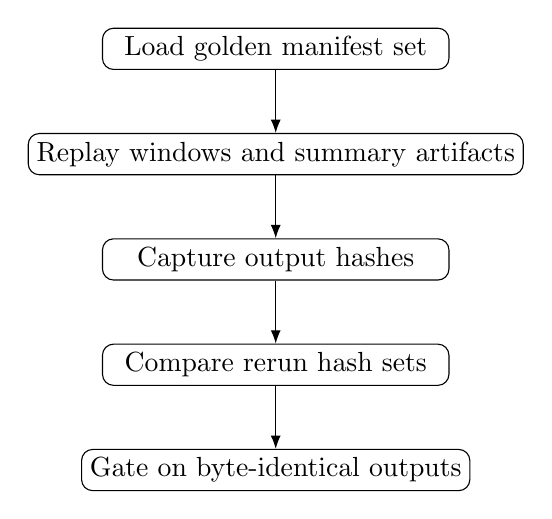
\begin{tikzpicture}[node distance=8mm and 12mm]
\node[box] (a) {Load golden manifest set};
\node[box, below=of a] (b) {Replay windows and summary artifacts};
\node[box, below=of b] (c) {Capture output hashes};
\node[box, below=of c] (d) {Compare rerun hash sets};
\node[box, below=of d] (e) {Gate on byte-identical outputs};
\draw[line] (a) -- (b);
\draw[line] (b) -- (c);
\draw[line] (c) -- (d);
\draw[line] (d) -- (e);
\end{tikzpicture}
\caption{Spike Deliverable 05: End-to-End Design Flow}
\end{figure}

\subsection*{Diagram B: Function Interaction and Attribute Flow}
\begin{figure}[H]
\centering
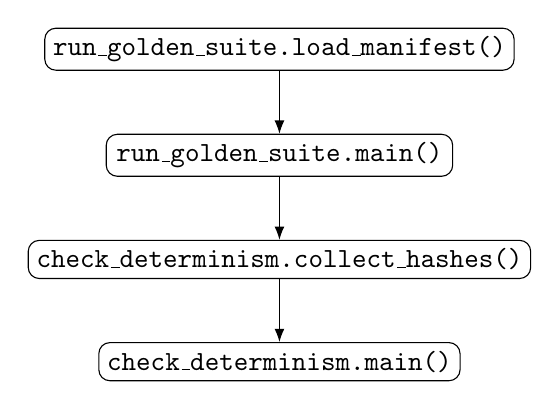
\begin{tikzpicture}[node distance=8mm and 12mm]
\node[box] (fa) {\texttt{run\_golden\_suite.load\_manifest()}};
\node[box, below=of fa] (fb) {\texttt{run\_golden\_suite.main()}};
\node[box, below=of fb] (fc) {\texttt{check\_determinism.collect\_hashes()}};
\node[box, below=of fc] (fd) {\texttt{check\_determinism.main()}};
\draw[line] (fa) -- (fb);
\draw[line] (fb) -- (fc);
\draw[line] (fc) -- (fd);
\end{tikzpicture}
\caption{Spike Deliverable 05: Function Interaction and Attribute Flow}
\end{figure}

\end{document}
